\documentclass[10pt,aspectratio=43]{beamer}

\usepackage{graphicx}
\graphicspath{{prebuilt_images/}}
\usepackage[sectionpages,
			rotationcw % clockwise, default is counterclockwise
			]{../sty/beamerthemeGlobalUniNA}

\usepackage[utf8]{inputenc}
\usepackage[english]{babel}
\usepackage[T1]{fontenc}
\usepackage{csquotes}
\usepackage{amsmath,amsfonts,amsthm,amssymb}

\usepackage[scaled]{beramono}
\usepackage[scale=1.05]{AlegreyaSans}
\usepackage{../sty/shortcuts_fb}

\usetikzlibrary{spy}
\usepackage[round]{natbib}
\bibliographystyle{plainnat}


%%%%%%%%%%%%%%%%%%%%%%%%%%%%%%%%%%%%%%%%%%%%%%%%%%%%%%%%%%%%%%%%%%%%%%%%%%%%%%%
% footnote setting: (1), (2), etc.
\usepackage{fnpct}

% Configure style for custom doubled line
\newcommand*{\doublerule}{\hrule width \hsize height 1pt \kern 0.5mm \hrule width \hsize height 2pt}

% Configure function to fill line with doubled line
\newcommand\doublerulefill{\leavevmode\leaders\vbox{\hrule width .1pt\kern1pt\hrule}\hfill\kern0pt }


\newcommand{\mytheorem}[2]{
\doublerulefill\ \framebox{\textbf{#1}}\ \doublerulefill
\vspace{0.1cm}

#2

\doublerulefill
}

\definecolor{javared}{rgb}{0.6,0,0} % for strings
\definecolor{javagreen}{rgb}{0.25,0.5,0.35} % comments
\definecolor{javapurple}{rgb}{0.5,0,0.35} % keywords
\definecolor{javadocblue}{rgb}{0.25,0.35,0.75} % javadoc
\definecolor{marron}{rgb}{0.64,0.16,0.16}
\definecolor{orange_js}{RGB}{230,159,0}

\newcommand{\mybold}[1]{\textcolor{marron}{\textbf{#1}}}
\newcommand{\cRm}[1]{\textsc{\romannumeral #1}}


%%%%%%%%%%%%%%%%%%%%%%%%%%%%%%%%%%%%%%%%%%%%%%%%%%%%%%%%%%%%%%%%%%%%%%%%%%%%%%%
%%%%%%%%%%%%%%%%%%%%%%%%%%%%%%%%%%%%%%%%%%%%%%%%%%%%%%%%%%%%%%%%%%%%%%%%%%%%%%%
% HEADER
%%%%%%%%%%%%%%%%%%%%%%%%%%%%%%%%%%%%%%%%%%%%%%%%%%%%%%%%%%%%%%%%%%%%%%%%%%%%%%%
%%%%%%%%%%%%%%%%%%%%%%%%%%%%%%%%%%%%%%%%%%%%%%%%%%%%%%%%%%%%%%%%%%%%%%%%%%%%%%%

\title[] %shown at the top of frames
{Ridge regularization: an essential concept in data science} %shown in title frame
\subtitle{Based on the article of Trevor Hastie 2020}

\date{04-2021} % explicitly set date instead of \today

\author[]%shown at the top of frames
{%shown in title frame
    {Bascou Florent} \\%
	{Lefort Tanguy}%
}

\institute[
]
{% is placed on the bottom of the title page
    University of Montpellier
}

\titlegraphic{% logos are put at the bottom-right part of the page
    
\includegraphics[width=2cm]{Logo.pdf}~ % also support multi-logos
    %
\includegraphics[width=2cm]{Logo.pdf}~ % up to 3 (after it gets messy)
    %
\includegraphics[width=2cm]{Logo.pdf} % if more, combine them in one image.
}

% You can also move it to where you want.
% This displays 3 logos above the title to the left-center-right
%\titlegraphic{%
%  \begin{picture}(0,0)
%    \put(18,165){\makebox(0,0)[rt]{
\includegraphics[width=2cm]{Logo.pdf}
%    \hspace{8em}
\includegraphics[width=2cm]{Logo.pdf}
%    \hspace{8em}
\includegraphics[width=2cm]{Logo.pdf}}}
%  \end{picture}}

\setbeamercolor{itemize subitem}{fg=red}
\setbeamertemplate{itemize subitem}[triangle]

%%%%%%%%%%%%%%%%%%%%%%%%%%%%%%%%%%%%%%%%%%%%%%%%%%%%%%%%%%%%%%%%%%%%%%%%%%%%%%%
%%%%%%%%%%%%%%%%%%%%%%%%       PLAN      %%%%%%%%%%%%%%%%%%%%%%%%%%%%%%%%%%%%%%
%%%%%%%%%%%%%%%%%%%%%%%%%%%%%%%%%%%%%%%%%%%%%%%%%%%%%%%%%%%%%%%%%%%%%%%%%%%%%%%

\begin{document}
\maketitle


%%%%%%%%%%%%%%%%%%%%%%%%%%%
% Table of contents
%%%%%%%%%%%%%%%%%%%%%%%%%%%
\begin{frame}{Content}{}
    \tableofcontents
\end{frame}

%%%%%%%%%%%%%%%%%%%%%%%%%%%%%%%%%%%%%%%%%%%
%%%%%%%%%%%%%% Introduction %%%%%%%%%%%%%%%
%%%%%%%%%%%%%%%%%%%%%%%%%%%%%%%%%%%%%%%%%%%

\section*{Introduction}
\begin{frame}{Introduction}{Ridge regularization}
truc
\end{frame}

%%%%%%%%%%%%%%%%%%%%%%
% Presentation
%%%%%%%%%%%%%%%%%%%%%%

\section{Linear model}
\begin{frame}{Ridge regularization}{Why use it?}
    Ordinary least squares:
    \[\hat\beta = \argmin_{\beta} \|y-X\beta\|_2^2 \Longleftrightarrow \hat \beta = (X^\top X)^{-1}X^\top y\]

    Problems that can happen:
    \begin{itemize}
        \item $X^\top X$ may be ill conditioned ($\kappa = \frac{\text{largest singular value}}{\text{smallest singular value}} \gg $ )
        \begin{onlyenv}<2->
            \begin{itemize}
                \item \color{red}{ Translate spectrum by $\lambda$ using $X^\top X + \lambda \mathrm{Id}.$}
            \end{itemize}
        \end{onlyenv}
        \item $p > n$ leads to infinite number of solutions for OLS.
        \begin{onlyenv}<2->
            \begin{itemize}
                \item \color{red}{ Add penalty to recover unicity.}
            \end{itemize}
        \end{onlyenv}
    \end{itemize}
    \begin{onlyenv}<3->
    \begin{block}{Ridge estimator}
        \[ \hat\beta_{ridge} = \argmin_{\beta} \|y-X\beta\|_2^2 \textcolor{red}{+ \lambda \|\beta\|^2_2} \Longleftrightarrow \hat \beta = (X^\top X \textcolor{red}{+ \lambda \mathrm{Id}})^{-1}X^\top y \]
    \end{block}
    \end{onlyenv}
\end{frame}

%%%%%%%%%%%%%%%%%%%%%%%%
% Kernel trick
%%%%%%%%%%%%%%%%%%%%%%%%
\section{Kernel trick}

\begin{frame}{Kernel trick}{When doing less is better}
    \begin{block}{Reduce the complexity}
        If $p>n$, $(X^\top X + \lambda \mathrm{Id})^{-1}\in\bbR^{p\times p}$ is costly.
        But we can actually only solve a $n\times n$ system thanks to the relation \emph{(proof with SVD)}:
        \[X^\top (X X^\top + \lambda \mathrm{Id})^{-1}y = (X^\top X + \lambda \mathrm{Id})^{-1}X^\top y\enspace.\]
    \end{block}
    \pause
    So we can write $\hat \beta = X^\top u$ with $u\in\bbR^{n}$. Denote $K=XX^\top$ the \textbf{Gram} matrix,
    \begin{align*}
        \hat y &= X\hat\beta = XX^\top u \\
               &= K(K + \lambda \mathrm{Id})^{-1}y
    \end{align*}

    \begin{itemize}
        \item New ridge problem smaller to solve.
        \item \textbf{Opens the door for a lot more!}
    \end{itemize}
\end{frame}

\begin{frame}{Kernel ridge regression}{Non linear relation}
Suppose $y_i=\varphi(X_i)$, then
 $\hat\varphi = \displaystyle\argmin_{\varphi\in\mathcal{H}} \|y-\varphi(X)\|^2_2 + \lambda \|\varphi\|_\mathcal{H}\enspace.$
 \begin{block}{Representer theorem}
        For $\mathcal{H}$ RKHS of kernel $K$ (symmetric!),
     \[\varphi = \sum_{i=1}^n \alpha_i K(x_i, \bullet)\enspace.\]
 \end{block}
 \pause
 The problem is now $\hat\alpha = \displaystyle\argmin_{\alpha} \|y-K\alpha\|^2_2 + \lambda \alpha^\top K \alpha$.
 \begin{itemize}
     \item first order conditions: $\nabla=(KK + \lambda K)\hat\alpha - Ky = 0$,
     \item solution: \[\textcolor{red}{\hat\alpha = (K+\lambda\mathrm{Id})^{-1}y} \enspace.\]
 \end{itemize}
\end{frame}


\begin{frame}{Kernel ridge regression}{Example with \texttt{KeOps} package}
    Gaussian kernel to estimate $\varphi(t) = t + t\cos(6t)$ on noised data,
\[K(x,y)=\exp\left\{-\gamma\|x - y\|^2_2\right\}, \gamma=\frac{1}{2\cdot 0.2^2} \enspace.\]
\begin{figure}
    \centering
    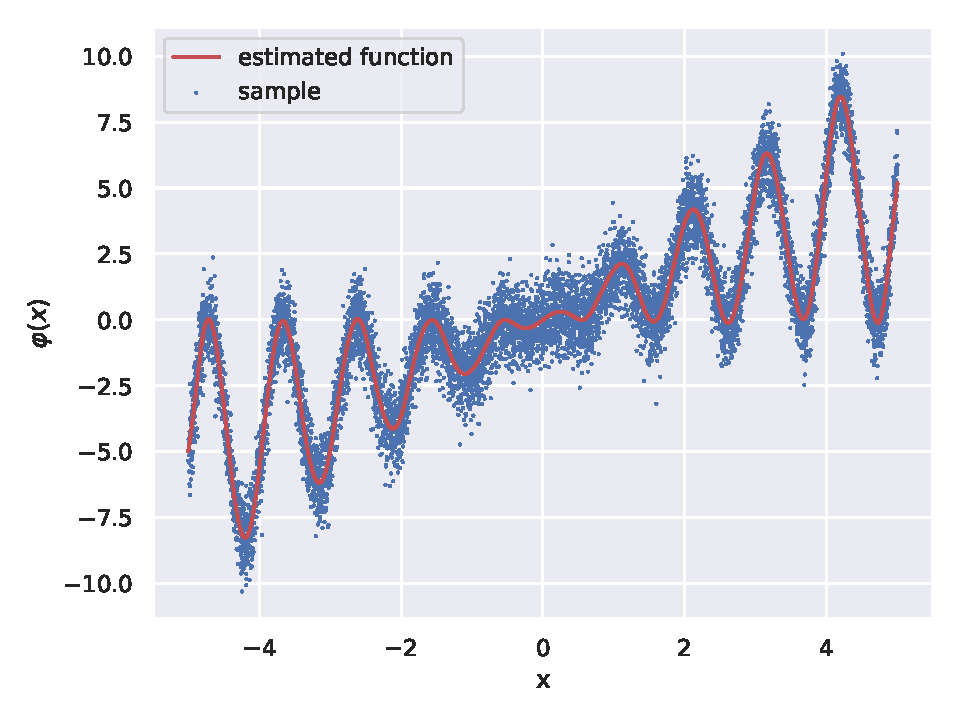
\includegraphics[scale=.45]{KRR.pdf}
\end{figure}
\end{frame}


%%%%%%%%%%%%%%%%%%%%%%%%
% Data augmentation
%%%%%%%%%%%%%%%%%%%%%%%%
\section{Data augmentation}

\begin{frame}{Data augmentation}{With images}
    \begin{center}
        Example of a small dog from CIFAR10 dataset
    \end{center}
    \begin{onlyenv}<1>
        \begin{figure}
            \centering
            
\includegraphics[scale=.6]{dog_cifar.pdf}
        \end{figure}
    \end{onlyenv}
    \begin{onlyenv}<2->
        \centering
    \begin{columns}[t]
        \column{.5\paperwidth}
        \begin{figure}
        \centering
        
\includegraphics[scale=.4]{dog_cifar.pdf}
        \end{figure}
        \column{.5\paperwidth}
        \centering
        \begin{onlyenv}<2>
            \begin{figure}
                \reflectbox{
\includegraphics[scale=.4]{dog_cifar.pdf}
                }
            \end{figure}
        \end{onlyenv}
        \begin{onlyenv}<3>
            \begin{figure}
                \vspace{-1.2cm}
            \hbox{\hspace{-3em}
            
\includegraphics[scale=.4, angle=30, origin]{dog_cifar.pdf}}
            \end{figure}
        \end{onlyenv}
    \end{columns}
    \end{onlyenv}
\end{frame}

\begin{frame}{Data augmentation}{And with cloud points?}
    \begin{figure}
        \centering
        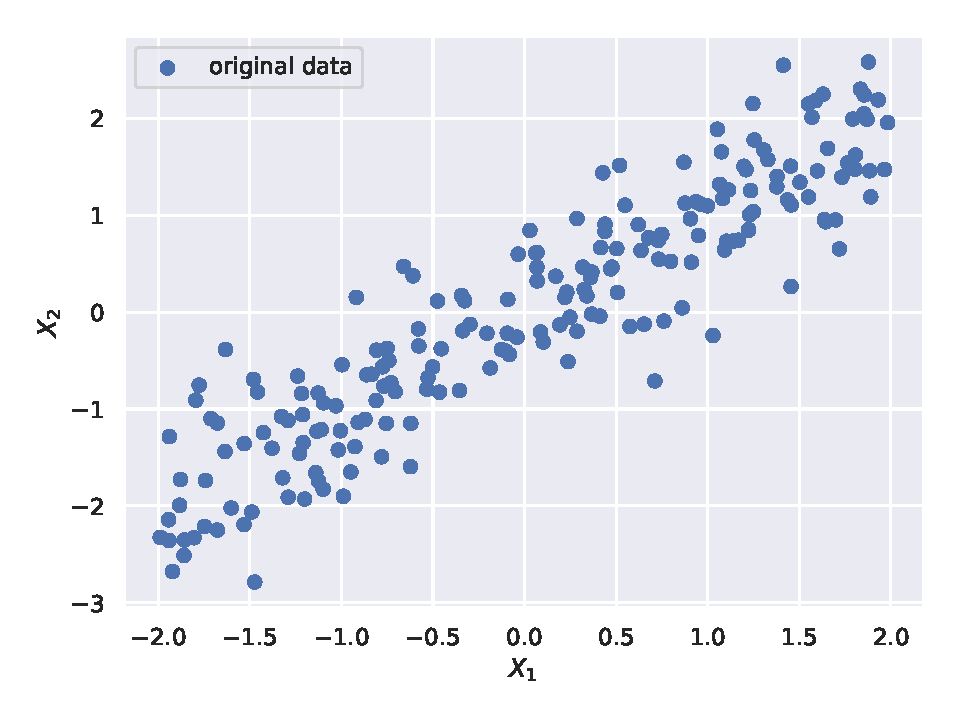
\includegraphics[scale=.5]{og_data_augm.pdf}
    \end{figure}
    \begin{itemize}
        \item \textbf{Goal:} Use the data we have to create new points,
        \item \textbf{But} can't flip it / make a small rotation, $\dots$
    \end{itemize}
\end{frame}

\begin{frame}{Data augmentation}{Perturbations on the cloud}
    One way to do so: create perturbated points from the data we have:
    \[x_{ij}=x_i + \varepsilon_{i,j}, \varepsilon_{ij}\sim\mathcal{N}\left(0, \frac{\lambda}{n}\mathrm{Id}\right), i\in[n], j\in[m]\enspace,\]
    \[\text{with associated response }y_{ij}=y_i\enspace .\]
    \vspace{-.5cm}
    \begin{columns}
        \begin{column}{.6\paperwidth}
            \begin{figure}
                \centering
                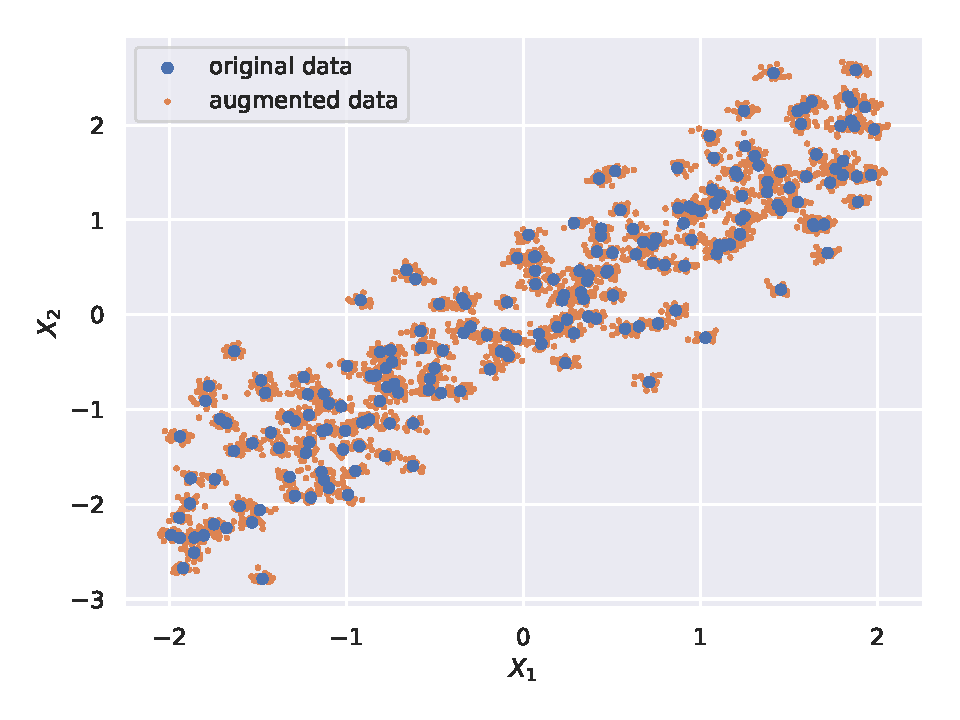
\includegraphics[scale=.35]{data_augmentation.pdf}
            \end{figure}
        \end{column}
        \begin{column}{.4\paperwidth}
            Added points compensate each other $$ \textcolor{red}{\sum_i\frac{1}{m}\sum_jx_{ij}x_{ij}^\top \simeq (XX^\top + \lambda \mathrm{Id})}$$
            OLS with $X^{augmented} \simeq$ Ridge with $X$
        \end{column}
    \end{columns}
\end{frame}

%%%%%%%%%%%%%%%%%%%%%%%%
% Double descent
%%%%%%%%%%%%%%%%%%%%%%%%

\begin{frame}{Double descent}{Over parametrization}
    Phenomenon observed in Deep Learning, Random Forests \dots
    \begin{onlyenv}<1>
        \begin{figure}
            \centering
            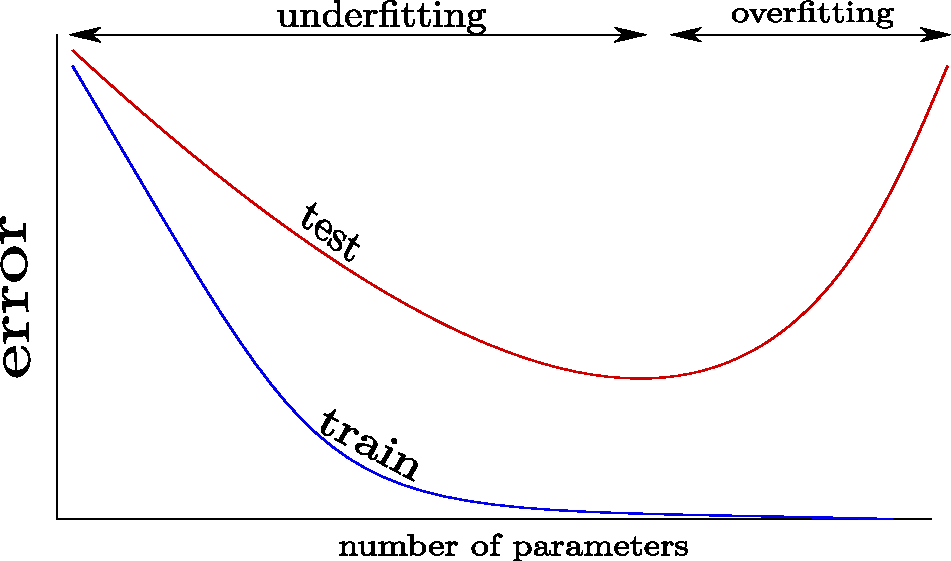
\includegraphics[scale=.6]{under_overfit_curves.pdf}
        \end{figure}
    \end{onlyenv}
    \begin{onlyenv}<2>
        \begin{figure}
            \centering
            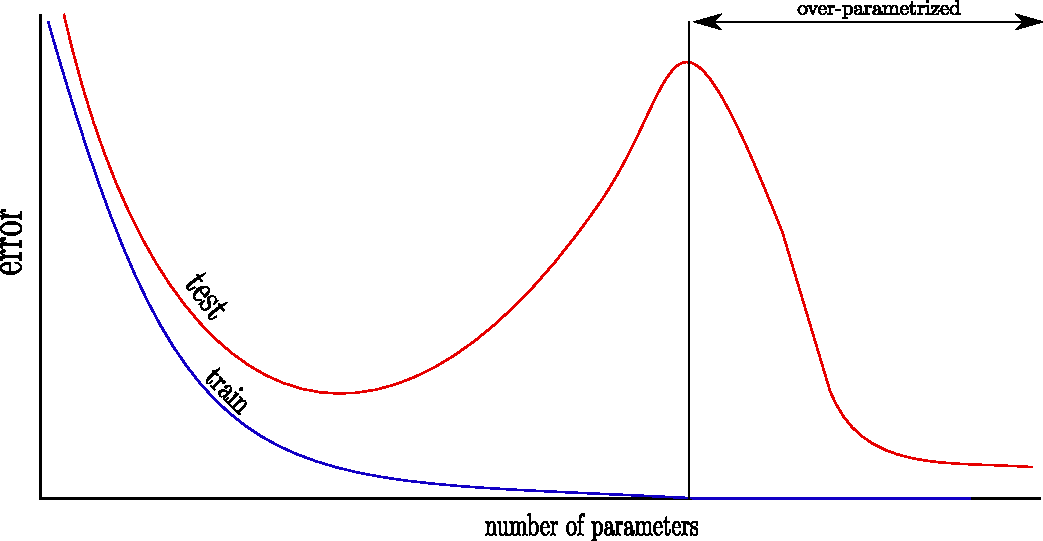
\includegraphics[scale=.6]{scheme_doubledescent.pdf}
        \end{figure}
    \begin{itemize}
        \item interpolate the data $\Longrightarrow$ $\ell_2$ norm of $\hat\beta$ is high,
        \item smaller $\ell_2$ norm for $\hat\beta$ generalize better and we keep zero training error.
    \end{itemize}
    \end{onlyenv}
\end{frame}

%%%%%%%%%%%%%%%%%%%%%%%%%%%%%%
% double descent with samples
%%%%%%%%%%%%%%%%%%%%%%%%%%%%%%

\begin{frame}{Double descent}{With samples \citep{nakkiran2020optimal}}
    In some cases ridge regularization can help get a monotonous error curve.
    \begin{columns}
        \begin{column}{0.46\textwidth}
            \begin{itemize}
                \item Isotropic data: $X\sim\mathcal{N}(O,\mathrm{Id})$,
                \item[]
                \item $n=1000$, $p=200$, $\|\beta^*\|_2=1$
                \item[]
                \item $y = X\beta^*+\varepsilon$ with $\varepsilon\sim \mathcal{N}(0, \sigma^2\mathrm{Id})$,
                \item $\lambda_{opt} = \sigma^2p$
            \end{itemize}
        \end{column}
        \begin{column}{0.7\textwidth}
            \begin{center}
             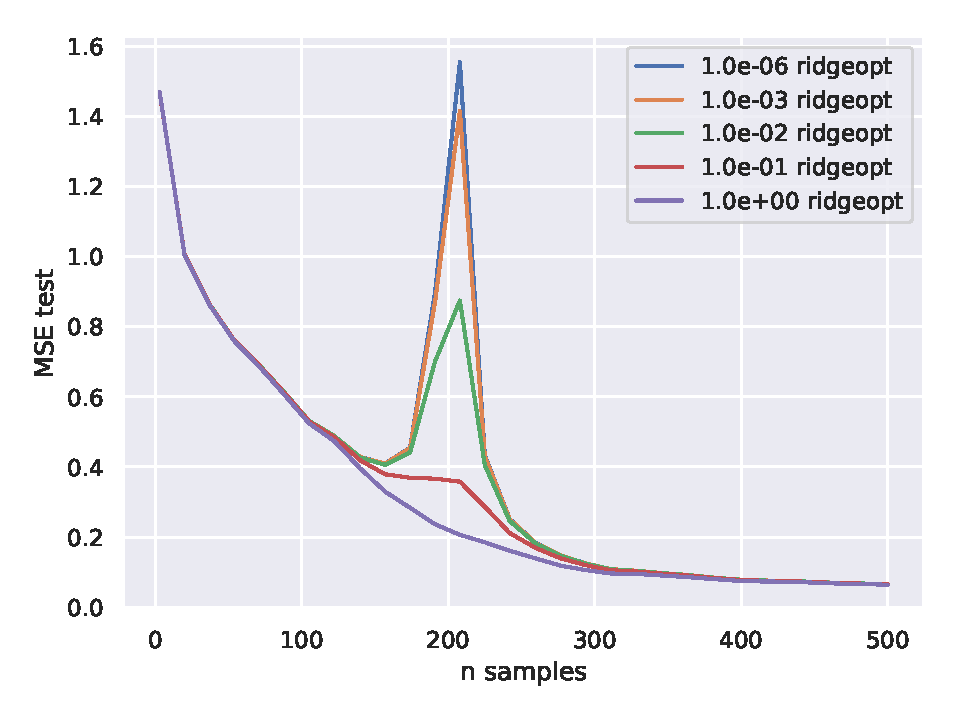
\includegraphics[width=1\textwidth]{double_descent.pdf}
             \end{center}
        \end{column}
        \end{columns}
    \begin{onlyenv}<2>
        \begin{block}{}
        We can achieve monotonic test error decrease with ridge regularization varying $p$ or $n$ for the linear models with isotropic covariates.
        \end{block}
    \end{onlyenv}
\end{frame}

%%%%%%%%%%%%%%%%%
% Biblio
%%%%%%%%%%%%%%%%%

\begin{frame}
    \bibliography{../sty/references.bib}

\end{frame}


\end{document}
